% THIS TEMPLATE IS A WORK IN PROGRESS

\documentclass[polish, a4paper]{article}
\usepackage[a4paper,left=3cm,right=3cm,top=3cm,bottom=1.5cm]{geometry}
\usepackage[T1]{fontenc}
\usepackage[polish]{babel}
\usepackage[utf8]{inputenc}
\usepackage{hyperref}
\usepackage{fancyhdr}
\usepackage{float}
\usepackage{graphicx}
\usepackage{titling}
\usepackage{caption}
\usepackage{pgfplots}
\usepackage{pgfplotstable}
\usepackage{filecontents}
\usepackage{csvsimple}
\usepackage{textcomp}
\usepackage{gensymb}
\usepackage{etoolbox}
%\usepackage{siunitx}
\graphicspath{ {./} }
\pagestyle{fancy}

\setlength{\droptitle}{-1in}

%\lhead{\includegraphics[width=0.2\textwidth]{nyush-logo.pdf}}

  \lhead{Maciej Kaszkowiak}
  \chead{Ćwiczenie 326}
  \rhead{Lab 4,
  151856}


%%%% PROJECT TITLE
\title{Badanie ogniwa fotowoltaicznego\\
        \Large \emph{Ćwiczenie nr 326 z działu Optyka}}

%%%% NAMES OF ALL THE STUDENTS INVOLVED (first-name last-name)
\author{Maciej Kaszkowiak, Lab 4, 151856}

\date{\vspace{-5ex}} %NO DATE


\begin{document}
\maketitle
%\thispagestyle{titlepage}

\section{Cel ćwiczenia}
Przeprowadzone ćwiczenie ma następujące cele:
\begin{enumerate}
\item{Zapoznanie się z podstawowymi wiadomościami na temat ogniw fotowoltaicznych. }
\item{Wyznaczenie:}
\begin{itemize}
\item{Zależności prądu fotoogniwa od natężenia oświetlenia;}
\item{Charakterystyk prądowo-napięciowych fotoogniwa dla różnych wartości natężenia oświetlenia;}
\item{Oporu wewnętrznego oświetlonego fotoogniwa.}
\end{itemize}
\end{enumerate}
\section{Wstęp teoretyczny}

Ogniwo fotowoltaiczne składa się z dwóch warstw półprzewodników, które są połączone metalicznymi elektrodami. Gdy na ogniwo pada światło o dostatecznie dużej energii, wewnątrz ogniwa zachodzi proces fotoelektryczny, w wyniku którego powstają pary dziura-elektron. Te nośniki ładunku są dyfuzyjnie przenoszone do złącza p-n. W zależności od strony, z której docierają, są tam odpowiednio zbierane. W ten sposób powstaje różnica potencjałów pomiędzy elektrodami, a po podłączeniu do odbiornika w zamkniętym obwodzie elektrycznym popłynie prąd elektryczny. Natężenie tego prądu jest w przybliżeniu proporcjonalne do natężenia oświetlenia fotoogniwa. Można określić charakterystyki prądowo-napięciowe oraz mocy od napięcia dla ogniwa fotowoltaicznego w zależności od natężenia światła. Maksymalny prąd zmienia się proporcjonalnie do jego oświetlenia, zaś maksymalna moc może zostać uzyskana, gdy rezystancja odbiornika jest równa rezystancji wewnętrznej ogniwa.



\section{Przebieg ćwiczenia}

\begin{enumerate}
\item{Włączyliśmy lampę i ustawiliśmy naprzeciwko niej detektor światła podłączony do luksomierza.}
\item{Wykonaliśmy pomiary natężenia oświetlenia L w funkcji odległości od źródła światła r w zakresie 20 - 90 cm (początkowo zmieniając odległość co 2 cm, potem co 5 cm a na koniec co 10 cm).}
\item{Odłączylismy detektor światła od luksomierza a następnie obróciliśmy. Połączyliśmy ogniwo fotowoltaiczne zgodnie ze schematem.}
\item{Na rezystorze dekadowym ustawiliśmy wartość $R_R$ = 0 $\Omega$, a następnie wykonaliśmy pomiary natężenia prądu I w funkcji odległości r od źródła światła w zakresie 20 - 90 cm.}
\item{Ustawiliśmy fotoogniwo w odległości r = 30 cm od lampy i wykonaliśmy pomiary natężenia prądu fotoogniwa od napięcia zmieniając rezystancję $R_R$. Pomiary te powtórzyliśmy dla odległości 35 cm oraz 45 cm.}
\end{enumerate}

\begin{figure}[H]
\centering
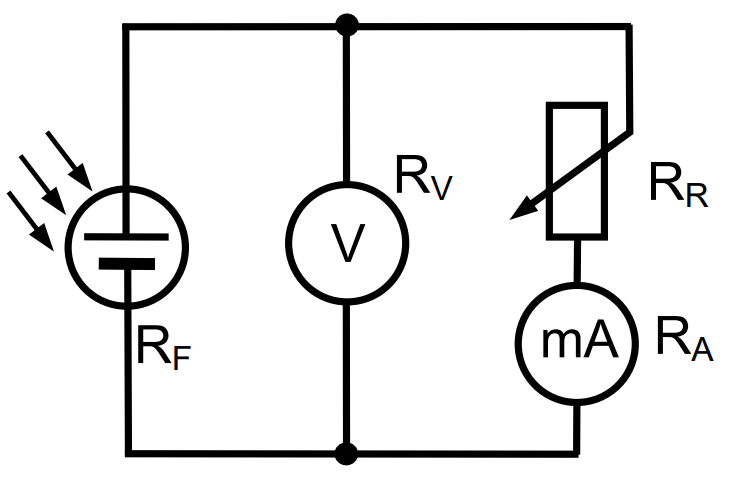
\includegraphics[width=0.5\textwidth]{uklad.png}
\caption{Schemat elektryczny obwodu pomiarowego}
\end{figure}

\section{Wyniki pomiarów}



\begin{table}[H]
    \centering
    \begin{tabular}{|l|l|l|l|l|}
    \hline
        \textbf{Dystans} & \textbf{Natężenie światła} & \textbf{Dokładność} & \textbf{Natężenie prądu} & \textbf{Dokładność} \\ 
        (cm) & (lux) & luksomierza & (mA) & amperomierza \\ \hline
        20 & 25800 & 100 & 70.0 & 0.1  \\ \hline
        22 & 21100 & 100 & 58.2 & 0.1 \\ \hline
        24 & 16440 & 10 & 48.8 & 0.1 \\ \hline
        26 & 14090 & 10 & 41.6 & 0.1 \\ \hline
        28 & 12030 & 10 & 36.1 & 0.1 \\ \hline
        30 & 10500 & 10 & 31.6 & 0.1 \\ \hline
        35 & 7750 & 10 & 23,6 & 0.1 \\ \hline
        40 & 5940 & 10 & 18,15 & 0.01 \\ \hline
        45 & 4770 & 10 & 14,73 & 0,01 \\ \hline
        50 & 3920 & 10 & 12,26 & 0,01 \\ \hline
        55 & 3330 & 10 & 10,46 & 0,01 \\ \hline
        60 & 2880 & 10 & 9,10 & 0,01 \\ \hline
        70 & 2080 & 10 & 7,16 & 0,01 \\ \hline
        80 & 1827 & 1 & 5,85 & 0,01 \\ \hline
        90 & 1535 & 1 & 4,91 & 0,01 \\ \hline
    \end{tabular}
    \caption{Pomiar natężenia światła zmierzonego przez luksomierz oraz natężenia prądu ogniwa fotowoltaicznego w zależności od dystansu od źródła światła.}
\end{table}

\begin{table}[H]
    \centering
        \csvreader[head to column names, 
        tabular=|l|l|l|l|,
        late after last line=\\\hline,
        late after line=\\\hline,
        table head=\hline Rezystancja $\Omega$ & Napięcie mV & Natężenie mA & Moc mW \\\hline]{zad2.csv}{}{\csuse{ohm} & \csuse{mv30} & \csuse{ma30} & \csuse{mw30}}
    \caption{Pomiar zależności natężenia prądu od napięcia dla r = 30cm, L = 10500 lux}
\end{table}

\begin{table}[H]
    \centering
        \csvreader[head to column names, 
        tabular=|l|l|l|l|,
        late after last line=\\\hline,
        late after line=\\\hline,
        table head=\hline Rezystancja $\Omega$ & Napięcie mV & Natężenie mA & Moc mW \\\hline]{zad2.csv}{}{\csuse{ohm} & \csuse{mv35} & \csuse{ma35} & \csuse{mw35}}
    \caption{Pomiar zależności natężenia prądu od napięcia dla r = 35cm, L = 7750 lux}
\end{table}


\begin{table}[H]
    \centering
        \csvreader[head to column names, 
        tabular=|l|l|l|l|,
        late after last line=\\\hline,
        late after line=\\\hline,
        table head=\hline Rezystancja $\Omega$ & Napięcie mV & Natężenie mA & Moc mW \\\hline]{zad2.csv}{}{\csuse{ohm} & \csuse{mv45} & \csuse{ma45} & \csuse{mw45}}
    \caption{Pomiar zależności natężenia prądu od napięcia dla r = 45cm, L = 4770 lux}
\end{table}

\section{Opracowanie wyników}

\begin{figure}[H]
\centering
\begin{tikzpicture}
\begin{axis}[
    width=\textwidth, height=0.6\textwidth,
    grid=major,
    xlabel={Odległość czujnika od źródła światła (cm)},
    ylabel={Natężenie światła (lux)},
   % legend style={at={(0.05,0.95)},anchor=north west},
    scaled ticks = false
]
% r_cm,,xd,I_mA
\addplot+[
    smooth,
    orange
] table[
    x = r_cm, col sep=comma,
    y = lux
] {zad1.csv};
\addlegendentry{Natężenie światła (lux)}
\end{axis}
\end{tikzpicture}
\caption{Zależność natężenia światła od odległości czujnika od źródła światła.}
\end{figure}

Zgodnie z teorią natężenie oświetlenia maleje z kwadratem
odległości od źródła światła $L = \frac{1}{r}$.


\begin{figure}[H]
\centering
\begin{tikzpicture}
\begin{axis}[
    width=\textwidth, height=0.6\textwidth,
    grid=major,
    xlabel={Natężenie światła (lux)},
    ylabel={Prąd (mA)},
    legend style={at={(0.05,0.95)},anchor=north west},
    scaled ticks = true
]
% r_cm,,xd,I_mA
\addplot+[
    smooth,
    orange
] table[
    x = lux, col sep=comma,
    y = I_mA
] {zad1.csv};
\addlegendentry{Prąd (mA)}
\end{axis}
\end{tikzpicture}
\caption{Zależność prądu ogniwa fotowoltaicznego w zależności od natężenia światła.}
\end{figure}

Możemy zauwazyć, że prąd ogniwa fotowoltaicznego rośnie liniowo w zależności od natężenia światła.

\begin{figure}[H]
\centering
\begin{tikzpicture}
\begin{axis}[
    width=\textwidth, height=0.6\textwidth,
    grid=major,
    xlabel={Napięcie (mV)},
    ylabel={Prąd (mA)},
    legend style={at={(0.05,0.05)},anchor=south west},
    scaled ticks = true
]
% ohm,ma30,mv30,ma35,mv35,ma45,mv45,mw30,mw35,mw45
\addplot+[
    smooth,
    orange
] table[
    x = mv30, col sep=comma,
    y = ma30
] {zad2.csv};
\addlegendentry{r = 30cm, L = 10500 lux}

\addplot+[
    smooth
] table[
    x = mv35, col sep=comma,
    y = ma35
] {zad2.csv};
\addlegendentry{r = 35cm, L = 7750 lux}

\addplot+[
    smooth
] table[
    x = mv45, col sep=comma,
    y = ma45
] {zad2.csv};
\addlegendentry{r = 45cm, L = 4770 lux}
\end{axis}
\end{tikzpicture}
\caption{Charakterystyki prądowo-napięciowe fotoogniwa
dla różnych wartości natężenia oświetlenia.}
\end{figure}

\begin{figure}[H]
\centering
\begin{tikzpicture}
\begin{axis}[
    width=\textwidth, height=0.6\textwidth,
    grid=major,
    xlabel={Napięcie (mV)},
    ylabel={Moc (mW)},
    legend style={at={(0.05,0.05)},anchor=south west},
    scaled ticks = true
]
% ohm,ma30,mv30,ma35,mv35,ma45,mv45,mw30,mw35,mw45
\addplot+[
    smooth,
    orange
] table[
    x = mv30, col sep=comma,
    y = mw30
] {zad2.csv};
\addlegendentry{r = 30cm, L = 10500 lux}

\addplot+[
    smooth
] table[
    x = mv35, col sep=comma,
    y = mw35
] {zad2.csv};
\addlegendentry{r = 35cm, L = 7750 lux}

\addplot+[
    smooth
] table[
    x = mv45, col sep=comma,
    y = mw45
] {zad2.csv};
\addlegendentry{r = 45cm, L = 4770 lux}
\end{axis}
\end{tikzpicture}
\caption{Zależność mocy od napięcia.}
\end{figure}

Gwałtowne skoki widoczne w kształcie wykresu odbiegające od teoretycznych założeń, w szczególności dostrzegalne dla odległości $r = 30cm$, wynikają z niedokładności aparatury pomiarowej. Punkty z gwałtownym spadkiem wynikają ze zmiany zakresu pomiarowego na mierniku, celem osiągnięcia możliwie najdokładniejszych wyników. 

W trakcie wykonywania pomiarów zanotowaliśmy szczególny przypadek w celu uwypuklenia powyższego problemu - zmierzone natężenie prądu wynosiło 2,3 mA na większym zakresie, natomiast 1,607 mA na mniejszym zakresie. Poszczególny przypadek miał miejsce przy ustawionym 200 Ohm rezystancji na rezystorze dekadowym i 45 cm odległości od źródła światła. Możemy zauważyć, że błąd bezwzględny wynosi 0,693 mA, natomiast błąd względny stanowi aż $43,1 \%$, przyjmując wartość natężenia z dokładniejszego zakresu pomiaru jako prawidłową.

\begin{figure}[H]
\centering
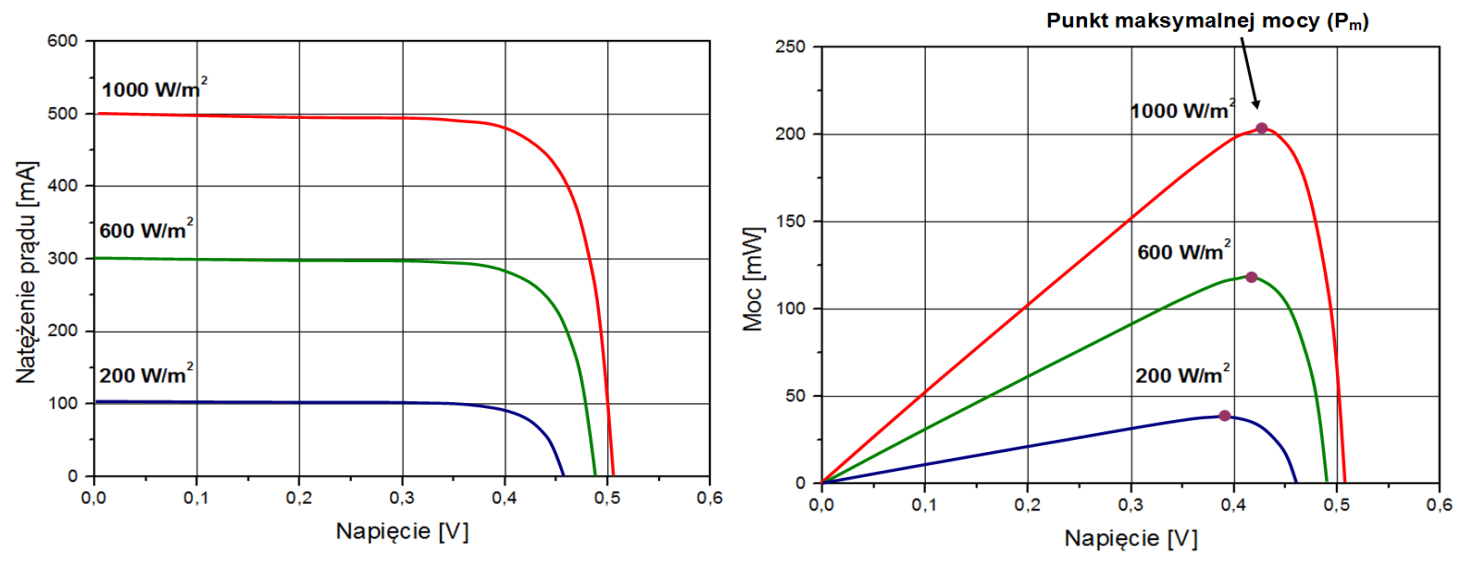
\includegraphics[width=\textwidth]{charakterystyki.png}
\caption{Teoretyczne charakterystyki prąd-napięcie oraz moc-napięcie przy różnym oświetleniu ogniwa fotowoltaicznego.}
\end{figure}

Pomijając gwałtowne skoki wynikające ze zmiany zakresu pomiarowego na mierniku, uzyskane pomiary zgadzają się z teoretycznymi założeniami. Możemy zaobserwować, że prąd fotoogniwa rośnie wraz z natężeniem oświetlenia padającego na fotoogniwo. Możemy również odczytać punkty największej mocy dla poszczególnych natężeń światła.

\begin{description}
    \item[r = 30cm, L = 10500 lux]{$U_{max} = 410 mV, P_{max} = 11.81 mW$}
    \item[r = 35cm, L = 7750 lux]{$U_{max} = 423 mV, P_{max} = 8.46 mW$}
    \item[r = 45cm, L = 4770 lux]{$U_{max} = 400 mV, P_{max} = 4.99 mW$}
\end{description}

Możemy również wyznaczyć rezystancję odbiornika $R_{odb}$, która w tym przypadku jest równa rezystancji wewnętrznej fotoogniwa $R_F$.

\begin{equation}
    R_{odb} = R_F = \frac{U_{max}^2}{P_{max}}
\end{equation}

\begin{description}
    \item[r = 30cm, L = 10500 lux]{$R_odb = 14.23 \Omega$}
    \item[r = 35cm, L = 7750 lux]{$R_odb = 21.15 \Omega$}
    \item[r = 45cm, L = 4770 lux]{$R_odb = 32.06 \Omega$}
\end{description}

\section{Wnioski}

Doświadczenie pozwoliło wykazać że prąd fotoogniwa rośnie liniowo wraz ze wzrostem natężenia
światła. Umożliwiło również wyznaczenie charakterystyk prądowo-napięciowych ogniwa fotowoltaicznego dla różnych wartości natężenia oświetlenia i zauważenie, że maksymalne napięcie zależy
od tego natężenia w niewielkim stopniu gdzie maksymalny prąd zmienia się znacząco. Dzięki wykresom moc-napięcie udało się wyznaczyć rezystancję wewnętrzną fotoogniwa dla poszczególnych
odległości od źródła światła.

\section{Bibliografia}

\begin{enumerate}
    \item {\emph{Badanie ogniwa fotowoltaicznego} (Krzysztof Łapsa)}
\end{enumerate}


\end{document}
